\documentclass{article}
\usepackage[utf8]{inputenc}

\title{Advanced Data Structures:\\Skip Lists}
\author{Constantino Gómez and Cristobal Ortega\\\{name.surname\}@est.fib.upc.edu}
\date{June 2016}

\usepackage{natbib}
\usepackage{float}
\usepackage{xcolor}
\usepackage{graphicx}
\usepackage{listings}
\usepackage[font=small,labelfont=it]{caption}
\usepackage{booktabs}
\usepackage[titletoc]{appendix}
\usepackage{hyperref}
\usepackage{amsmath}



%Use it for listings to not be split when pagebreaks appear
\floatstyle{plain} % optionally change the style of the new float
\newfloat{Code}{H}{myc}
\lstdefinestyle{myC}{
  frame=single,
  captionpos=b,
  belowcaptionskip=1\baselineskip,
  breaklines=true,
  xleftmargin=\parindent,
  morekeywords={nullptr, key},
  language=C++,
  numbers=left,
  numbersep=5pt,
  showstringspaces=false,
  basicstyle=\fontsize{8}{10}\ttfamily,
  keywordstyle=\bfseries\color{blue}\ttfamily,
  commentstyle=\itshape\color{gray}\ttfamily,
  identifierstyle=\color{black},
  stringstyle=\color{red},
}

\begin{document}

\maketitle

\section{Implementation}
Our implementation of the skip lists are based on the material provided in the Advanced Data Structures course\citep{ads:slides}, therefore our skip list class is composed of nodes with the following characteristics:

\begin{itemize}
    \item integer key
    \item string value
    \item List of nodes corresponding to the different levels
\end{itemize}

\begin{Code}
    \begin{lstlisting}[caption=Class Node, style=myC]
    struct Node {
        int key;
        std::string value;
    
        std::vector<Node*> _next;
        Node (int k, const std::string& v, int level);
    };
    \end{lstlisting}
\end{Code}

For simplification, we have fixed the data type our skip lists can work with. In our implementation, all the keys are Integers and the values are Strings.\\

Also, instead of having a lists of pointers to nodes representing the different levels we can have, we simplified this mechanism as a vector with a maximum height (this has a limitation: we cannot have more levels than \textit{MAX\_LEVELS}).\\

Even with these changes, we used the material provided in the course as a base to code the functions we had to develop for the assignment and the additional functions we consider that are needed to the basic usage of the skip lists. Our implementation includes this following data members and functions:

\begin{itemize}
    \item void insert (int key, string value): as in any data structure we need to be able to insert new elements 
    \item void erase (int key): as in any data structure we need to be able to delete elements 
    \item bool contains (int key): in order to check if inserts are done correctly, we coded this function to check if \textit{key} is in the list
    \item string find (int key): we need to retrieve information from the data structure, even more, for this assignment we need to be able to measure the cost of finding
    \item int total\_search\_cost(): requirement of the assignment
    \item int number\_pointers(): requirement of the assignment
    \item int randomLevel(): because of how skip lists work we need to provide a random function to get the height of new nodes created
    \item int getLevel(vector\textless Node*\textgreater \& x): because the levels can differ we need an auxiliary function to evaluate the height of the given \textit{key}
    \item void print(): coded to be able to debug the data structure, it prints the lowest level (the most complete list) of the data structure and prints for each \textit{key} its level.
\end{itemize}

The different functions that go through the data structure (insert, erase, contains, find, etc.) are almost the same as the snippet shown in the material \citep{ads:slides}:


\begin{Code}
    \begin{lstlisting}[caption=Snippet to iterate through the skip list, style=myC]
      int l = actualLevel;
      while ( l>=0 ){
        if (x->_next[l] == nullptr || key <= x->_next[l]->key){
          to_update[l] = x;
          --l;
        }
        else {
          x = x->_next[l];
        }
      }
      x = x->_next[0];
    \end{lstlisting}
\end{Code}

With the snippet shown above we are able to get the position where the pair \textless \textit{key, value}\textgreater \ should be or should not be placed. After, finding the position and depending on what function was called we will do different things: return true if it exists, return the value, etc.\\
\\
The code of our skip lists implementation can be obtained from the appendixes of this work and also from our Github repository\citep{github:cristobal}.

\section{Experimental framework}

We describe the hardware characteristics of the machine where this data structure has been tested in Table \ref{table:specs}


\begin{table}[H]
    \centering
    \begin{tabular}{@{}ll@{}}
    \toprule
    Processor & Intel(R) Core(TM) i7-4600U \\
    Frequency & 2.1 GHz                    \\
    L1        & 64 KB                      \\
    L2        & 512 KB                     \\
    Memory    & 8 GB                       \\ \bottomrule
    \end{tabular}%
    \caption{Machine specifications}
    \label{table:specs}
\end{table}

We use a main program to execute several tests and measure the different metrics required for the assignment:
\begin{description}
    \item[Total cost of searching.]{We need to search for every element and compute its cost, C(n,k), and for the total cost it will be the addition of all individual costs of searching: $C(n) = \sum_{k=1}^{n}C(n,k)$}
    \item[Total usage of memory.]{We can count the number of pointers that we use for storing the data, at the end we would need to multiply each pointer to its real size on memory (key, value, etc.)}
\end{description}

In order to obtain these metrics values, we added auxiliar functions: \textit{total\_search\_cost} and \textit{number\_pointers}. With those values, we analyze and compare different skip lists configurations varying the size \textit{(N)} and the probability to copy the node to the upper level \textit{(p)}\\
\\
\textit{Comment: we repeat each experiment 50 times and get the average to minimize the impact of outliers in our results.}\\

\section{Results} \label{sec:results}
In this section we discuss the results obtained experimenting with our implementation of skip lists.\\
\\
From now on, we use the term skip list size to refer to the total number of elements contained in a skip list. In figure \ref{fig:search_cost} we show the total search cost in seconds ($C(n) = \sum_{k=1}^{n}C(n,k)$) varying the size of skip list and \textit{p} factor; meaning that for each size of skip lists ranging from 1K to 10K with 1K increase,  we try different [0 to 1; 0.1++] values of \textit{p} factor. The \textit{p} factor determines the probability of copying an element to an upper level.
\\
\\
We easily identify different trends: 

\begin{figure}[H]
  \begin{center}
    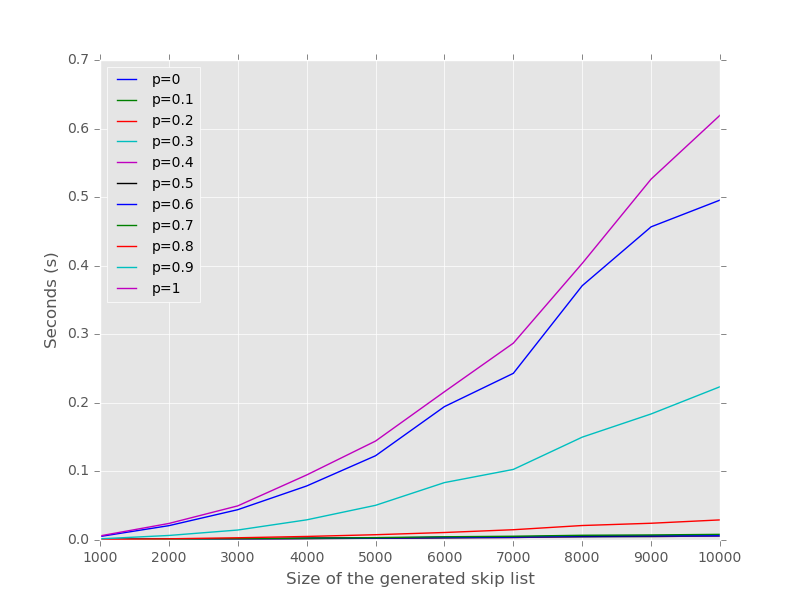
\includegraphics[width=0.8\textwidth]{imgs/time.png}
    \caption{Total search cost for different sizes and \textit{p}}
    \label{fig:search_cost}
  \end{center}
\end{figure}


\begin{itemize}
    \item For extreme values of \textit{p} searches become slower. The reason for this behavior is due to how we build the skip list, with extreme values of \textit{p} we get a \textit{flat} list:
    \begin{itemize}
        \item At \textit{p = 0},  elements are never copied to an upper level; resulting in a list with elements only in the 1st level.
        \item At \textit{p = 1}, elements are \textbf{always} copied to an upper level (for this reason we have a \textit{MAX\_LEVELS}, so our data structure does not grow to infinity).
    \end{itemize}
    \item We focus on non-extreme \textit{p} values on figure \ref{fig:search_cost2}. As we see, all lines exhibit very similar behavior in terms of performance.
\end{itemize}

\begin{figure}[H]
  \begin{center}
    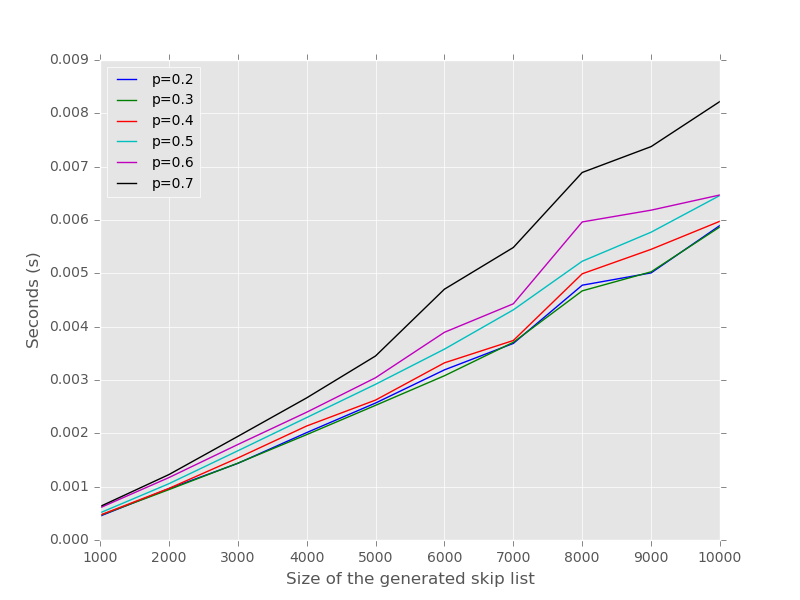
\includegraphics[width=0.8\textwidth]{imgs/time2.png}
    \caption{Total search cost for different sizes and \textit{p} (without extreme values of \textit{p})}
    \label{fig:search_cost2}
  \end{center}
\end{figure}

To reason about memory space consumption, for different \textit{p} and skip list size values, we measured the total number of pointers allocated in each skip list configuration. Figure \ref{fig:num_pointers} shows our results varying p and skip list size the same way as in the previous experiment.\\
\\
We observe that for high values of \textit{p} we are using more pointers, therefore more memory space. This has an easy explanation: a higher value of \textit{p} more the possibility to copy the element to an upper level, and in consequence we will have more copies of the element (that as seen in figure \ref{fig:search_cost} can be useful for reducing the search cost).

\begin{figure}[H]
\begin{center}
    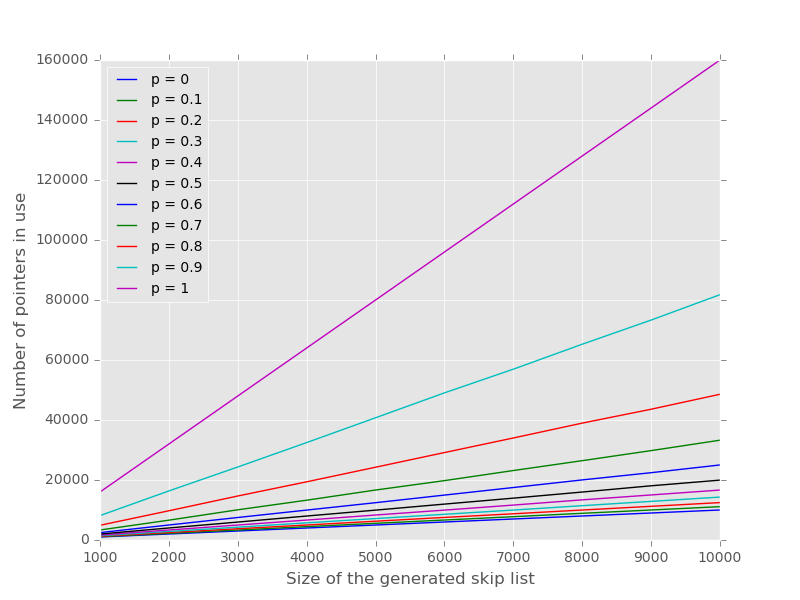
\includegraphics[width=0.8\textwidth]{imgs/pointers.png}
    \caption{Total number of used pointers for different sizes and \textit{p}}
    \label{fig:num_pointers}
  \end{center}
\end{figure}

In this case, we filter high values of \textit{p} because they are not representative (see figure \ref{fig:num_pointers2}).

\begin{figure}[H]
\begin{center}
    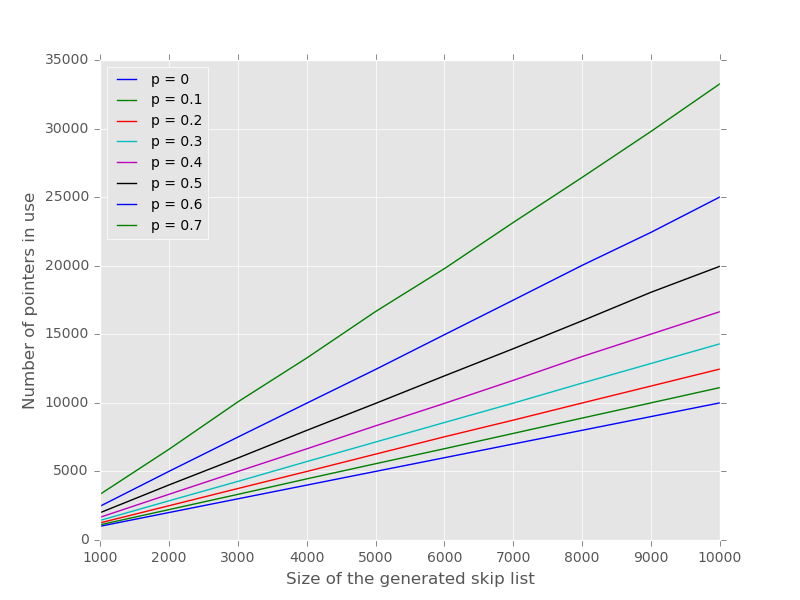
\includegraphics[width=0.8\textwidth]{imgs/pointers2.png}
    \caption{Total number of used pointers for different sizes and \textit{p} (without high values of \textit{p})}
    \label{fig:num_pointers2}
  \end{center}
\end{figure}

\subsection{Theoretical comparison}
Following, we compare our implementation against the theorical skip list characteristics:

\begin{itemize}
    \item Total Search cost: $n\times\log n$
    \item Space in memory: $n$
\end{itemize}

We compare search cost in figure \ref{fig:search_cost_teorical} and space in memory in figure \ref{fig:num_pointers_teorical}. Both of them are in logarithmic scale to see better how our implementation has the same growing shape. They only differ in a ratio, probably because on how we implemented our version.

\begin{figure}[H]
  \begin{center}
    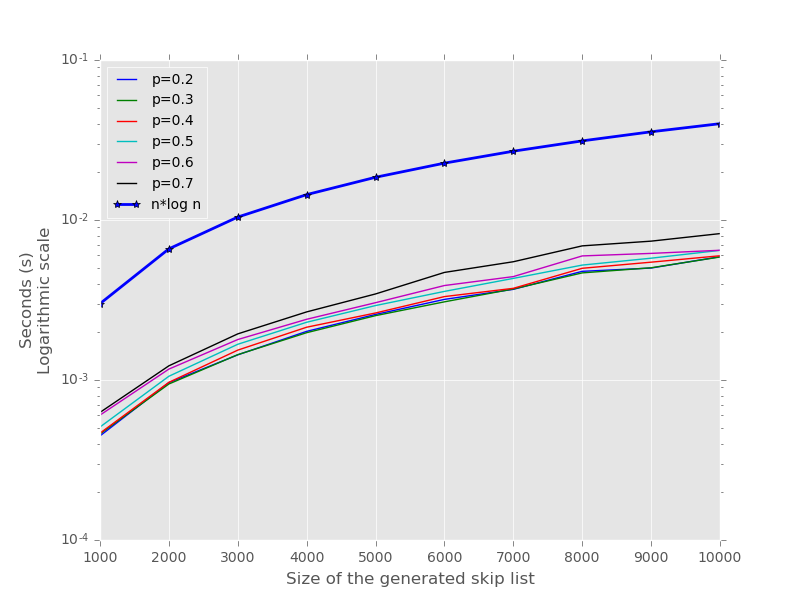
\includegraphics[width=0.8\textwidth]{imgs/time_teorical.png}
    \caption{Total search cost for different sizes and \textit{p} (without extreme values of \textit{p}) and the theoretical function}
    \label{fig:search_cost_teorical}
  \end{center}
\end{figure}

\begin{figure}[H]
\begin{center}
    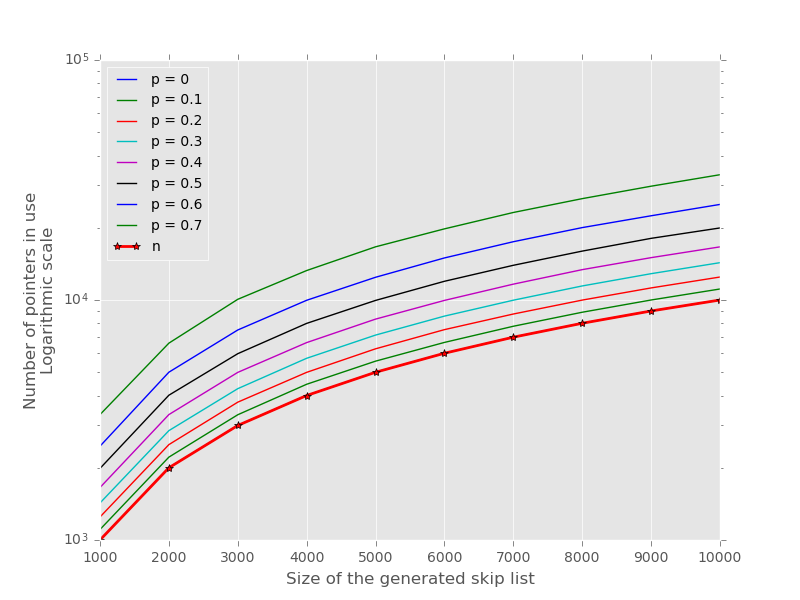
\includegraphics[width=0.8\textwidth]{imgs/pointers_teorical.png}
    \caption{Total number of used pointers for different sizes and \textit{p} (without high values of \textit{p}) and the theorical function}
    \label{fig:num_pointers_teorical}
  \end{center}
\end{figure}

Additionaly, we tested how the probability \textit{p} affects our total search cost, the experiments realized are represented in the figure \ref{fig:limit}.
We made 2 large skip lists (n=10000 and n=50000) and compared their total search cost against the theoretical one represented as the function: $\frac{-1}{q \ln q}$.

\begin{figure}[H]

\begin{center}
    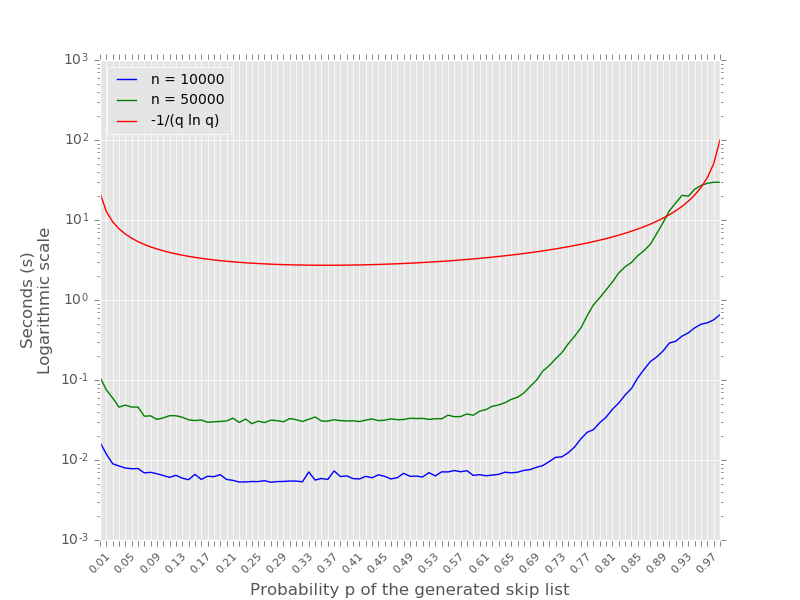
\includegraphics[width=0.8\textwidth]{imgs/limit_q.png}
    \caption{Total search cost for different probabilities \textit{p}}
    \label{fig:limit}
  \end{center}
\end{figure}

As we can observe in figure \ref{fig:limit} it seems to be a global minimum for the total search cost, in the next table \ref{table:limit} we wrote down the probability \textit{p} that offers the most performance in terms of total search cost, in the table we can see that we are close to the minimum theoretical (even lower), this may be an artifact on the implementation or the experiments:  (1) our implementation can have corner cases where we are not getting the good node, even we have debug several cases (coded in the main.cpp (appendix \ref{code:main})) or (2) our experiments are very short in repetitions, we had to lower the repetitions for the case when \textit{N=50000} due to high execution time, therefore we can be seeing problems with extreme cases that lower our average time.\\

\begin{table}[H]
\centering
\begin{tabular}{@{}cc@{}}
\toprule
N           & \begin{tabular}[c]{@{}l@{}}p with minimum\\  total search cost\end{tabular} \\ \midrule
10000       & 0.33                                                                        \\
50000       & 0.28                                                                            \\
Theoretical & 0.37 ($\frac{1}{e}$)                                                           \\ \bottomrule
\end{tabular}
\caption{Probability \textit{p} that offers the best total search cost}
\label{table:limit}
\end{table}

\newpage
\section{Conclusion}
After finalizing this assignment, we do have some final remarks to conclude.\\
Skip lists seem a good alternative to that data structures that are more often used: their behavior it is similar to those alternatives (and also the idea behind them it is a quite interesting one) as we have proven in the previous section \ref{sec:results}\\
Actually, we had a great time implementing this data structure because we never heard about them before and as we already said, we think this data structure is interesting.
And, overall we think we are close enough to the theoretical values and that makes our implementation good to be used in the future.


\bibliographystyle{plain}
\bibliography{references.bib}

\newpage

\appendix

\section{skipList.hpp}
\begin{lstlisting}[caption=Code from file skipList.hpp, style=myC]
#ifndef SKIP_LIST_H
#define SKIP_LIST_H
#include <stdio.h>
#include <stdlib.h>
#include <time.h>
#include <iostream>
#include <string>
#include <sstream>
#include <vector>
#include <algorithm>
#include <random>
#include <cmath>
#include <chrono>
#include <sys/time.h>
#include <iomanip>
#include <unistd.h>

struct Node {
    int key;
    std::string value;
    std::vector<Node*> _next;
    
    Node (int k, const std::string& v, int level);
};

class skipList {
  public:
    skipList();
    skipList(double probability);
    ~skipList();

    void print();

    void insert (int key, std::string v);
    void remove (int key);
    std::string find(int key);
    bool contains (int key);

    //Support for ADS
    long long total_search_cost();
    int number_pointers();


    Node* head;
    Node* NIL;

  private:
    int maxLevel;
    double prob;
    int _height;
    long long _lastFind;
    long long _totalSearchCost;

    int randomLevel();
    int getLevel (std::vector<Node*>& x);
};

#endif
\end{lstlisting}


\section{skipList.cpp}
\begin{lstlisting}[caption=Code from file skipList.cpp, style=myC]
#include "skipList.hpp"

skipList::skipList() {
  this->prob = 0.5;
  this->maxLevel = 16;
  int key = std::numeric_limits<int>::min();
  head = new Node(key, "head", maxLevel);

  key = std::numeric_limits<int>::max();
  NIL = new Node(key, "NIL", maxLevel);

  for(unsigned int i = 0; i < maxLevel; i++) {
    head->_next[i] = NIL;
  }
  //std::cout << "Created" << std::endl;
  _height = 0;
  _lastFind = 0;
  _totalSearchCost = 0;
}

skipList::skipList(double probability) {
  this->prob = probability;
  this->maxLevel = 16;
  int key = std::numeric_limits<int>::min();
  head = new Node(key, "head", maxLevel);

  key = std::numeric_limits<int>::max();
  NIL = new Node(key, "NIL", maxLevel);

  for(unsigned int i = 0; i < maxLevel; i++) {
    head->_next[i] = NIL;
  }
  //std::cout << "Created" << std::endl;
  _height = 0;
  _lastFind = 0;
  _totalSearchCost = 0;
}

Node::Node(int k, const std::string& v, int level) {
  key = k;
  value = v;
  for(unsigned int i = 0; i< level; ++i)
    _next.emplace_back(nullptr);
}

skipList::~skipList() {
  //MEMORY IS FREE! :D
  //But leakage problem is real :(
}


int skipList::getLevel( std::vector<Node*>& x ) {
  int aux = 0;
  int max = std::numeric_limits<int>::max();

  //We are in NIL status
  if (x[0]->key == max) {
    return aux;
  }

  int result;
  for (unsigned int i = 0; i < x.size(); ++i) {
    if (x[i] != nullptr && x[i]->key != max){
      ++aux;
    }else{
      break;
    }
  }
  return aux;
}

void skipList::print() {
  std::cout << "==========" << std::endl;
  std::cout << "Printing information about skip list" << std::endl;
  std::cout << "Probability: " << this->prob << " Max Level: " \
    << this->maxLevel << std::endl;


  Node* list = head;

  std::cout << "HEAD address: " << &head << std::endl;
  std::cout << "NIL address: " << &NIL << std::endl;

  std::cout << "===PRINT AS A VECTOR===" << std::endl;
  while (list->_next[0] != nullptr) {
    std::cout << "Address: " << &list->_next[0] << std::endl;
    std::cout << "Key: " << list->_next[0]->key \
      << " value: " << list->_next[0]->value \
      << " level: " << getLevel(list->_next) \
      << std::endl;

    list = list->_next[0];

  }





  std::cout << "==========" << std::endl;

}


void skipList::insert (int key, std::string v) {
  //std::cout << "Inserting Key: " << key << " with value: " << v << std::endl;
  int actualLevel = getLevel(head->_next);
  std::vector<Node*> to_update(head->_next);

  Node* x = head;

  int l = actualLevel;
  while ( l>=0 ){
    if (x->_next[l] == nullptr || key <= x->_next[l]->key){
      to_update[l] = x;
      --l;
    }
    else {
      x = x->_next[l];
    }
  }

  if ( x->_next[0] == nullptr || x->_next[0]->key != key) {
   int level = randomLevel();
   int height = getLevel(to_update);
   if ( level > height ) {
     for (unsigned int i = height; i < level - 1; ++i) {
      to_update[i] = head;
     }
   }
   x = new Node(key, v, level);

    for (unsigned i = 0; i < level; ++i) {
      x->_next[i] = to_update[i]->_next[i];
      to_update[i]->_next[i] = x;
    }
  }
  else {
    x->_next[0]->value = v;
  }

  return;
}

void skipList::remove (int key) {
  //std::cout << "Removing Key: " << key << std::endl;
  int actualLevel = getLevel(head->_next);
  std::vector<Node*> to_update(head->_next);

  Node* x = head;

  int l = actualLevel;
  while ( l>=0 ){
    if (x->_next[l] == nullptr || key <= x->_next[l]->key){
      to_update[l] = x;
      --l;
    }
    else {
      x = x->_next[l];
    }
  }
  x = x->_next[0];

  if ( x == nullptr) {
    //we did something wrong
    std::cout << "Removing a nullptr" << std::endl;
    return; //we like return in voids
  }

  if (x->key == key) {
    int height = getLevel(x->_next);
    for (int i = 0; i <= to_update.size(); i++) {
      if( to_update[i]->_next[i] != x)
        break;

      to_update[i]->_next[i] = x->_next[i];
    }
    delete x;

  }

}

std::string skipList::find(int key) {
  timeval start,end;
  gettimeofday(&start,NULL);
  
  int actualLevel = getLevel(head->_next);
  std::vector<Node*> to_update(head->_next);

  Node* x = head;

  int l = actualLevel;
  while ( l>=0 ){
    if (x->_next[l] == nullptr || key <= x->_next[l]->key){
      to_update[l] = x;
      --l;
    }
    else {
      x = x->_next[l];
    }
  }
  x = x->_next[0];



  std::string result;
  if ( x == nullptr) {
    //we did something wrong
    std::cout << "Searching in a nullptr :D" << std::endl;
    result = "";
  }

  if (x->key == key) {
    result = x->value;
  } else {
    result = "";
  }

  gettimeofday(&end,NULL);
  this->_lastFind = (end.tv_sec - start.tv_sec)*1000000 + (end.tv_usec - start.tv_usec);
  this->_totalSearchCost += this->_lastFind;

  return result;
}

bool skipList::contains (int key) {
  //std::cout << "Searching Key: " << key << std::endl;
  int actualLevel = getLevel(head->_next);
  std::vector<Node*> to_update(head->_next);

  Node* x = head;

  int l = actualLevel;
  while ( l>=0 ){
    if (x->_next[l] == nullptr || key <= x->_next[l]->key){
      to_update[l] = x;
      --l;
    }
    else {
      x = x->_next[l];
    }
  }
  x = x->_next[0];

  if ( x == nullptr) {
    //we did something wrong
    std::cout << "Searching in a nullptr :D" << std::endl;
    return false;
  }

  if (x->key == key) {
    return true;
  } else {
    return false;
  }
  return true;
}

int skipList::number_pointers() {
  Node* list = head;
  //std::cout << "Counting pointers" << std::endl;

  //Initialize to 1 because of the HEAD pointer needed to have referenced
  // the skip list, even empty, we need it
  int total_pointers = 1;
  while (list->_next[0] != nullptr) {
    total_pointers += getLevel(list->_next);

    list = list->_next[0];
  }
  return total_pointers;

}

long long skipList::total_search_cost(){
  return this->_totalSearchCost;
}

//PRIVATE
int skipList::randomLevel() {
  //std::cout << "randomLevel generator" << std::endl;
  //int aux = 1;
  //srand ((unsigned)time(NULL));
  //bool cond = ((double)std::rand() / RAND_MAX) < this->prob;
  ////while (cond || (aux < maxLevel - 1) ) {
    ////++aux;
    ////cond = ((double) std::rand() / RAND_MAX) < this->prob;
  ////}
  //while ((((double)std::rand() / RAND_MAX)) < prob && std::abs(aux) < maxLevel)
    //++aux;

  int aux = 1;
  std::random_device rd;
  std::default_random_engine rng(rd());
  std::uniform_real_distribution<float> uniform_dist(0,1);
  float random = uniform_dist(rng);
  bool cond = random < this->prob;
  while ( cond && std::abs(aux) < maxLevel ) {
    random = uniform_dist(rng);
    cond = random < this->prob;
    ++aux;
  }
  //std::cout << "RANDOM LEVEL: " << aux << std::endl;
  return aux;
}


\end{lstlisting}

\section{main.cpp (launch experiments and collect data)} \label{code:main}
\begin{lstlisting}[caption=Code from file main.cpp, style=myC]
#include "skipList.hpp"
#include <stdio.h>

#define REPETIONS 50

void benchmark(int size) {

  std::cout << "0";
  for (double p = 0.1; p <= 1; p+=0.1) {
    std::cout << ":" << p;
  }
  std::cout << std::endl;

  float  n_pointers[11];
  float  n_cost[11];
  for (int i = 0; i < 11; i++){
    n_pointers[i] = 0;
    n_cost[i] = 0;
  }

  int pos = 0;
  for (int j = 0; j < REPETIONS; j++) {
    pos = 0;
    for (double p = 0; p <= 1; p+=0.1) {
      skipList sl(p);

      //fill skip list
      for (unsigned int i = 0; i < size; i++) {
        std::stringstream ss;
        ss << i;
        sl.insert(i,ss.str());
      }

      //search in find list for cost
      for (unsigned int i = size - 1; i > 0; i--) {
        std::string aux = sl.find(i);
      }
      n_cost[pos] += sl.total_search_cost();
      /*std::cout << sl.total_search_cost();*/
      /*if (p+0.1 < 1.0 )*/
        /*std::cout << ":";*/
      /*else std::cout << std::endl;*/

      /*n_pointers.push_back(sl.number_pointers());*/
      n_pointers[pos] += sl.number_pointers();
      ++pos;
    }
  }
  for(int i = 0; i < 11; ++i) {
    std::cout << n_cost[i]/REPETIONS;
    if (i+1 < 11)
      std::cout << ":";
    else
      std::cout << std::endl;

  }
  for(int i = 0; i < 11; ++i) {
    std::cout << n_pointers[i]/REPETIONS;
    if (i+1 < 11)
      std::cout << ":";
    else
      std::cout << std::endl;

  }


}

void test() {
  int size = M;
  double p = 0.75;

  skipList sl(p);

  //fill skip list
  for (unsigned int i = 0; i < size; i++) {
    std::stringstream ss;
    ss << i;
    sl.insert(i,ss.str());
  }

  //search in find list
  for (unsigned int i = size - 1; i > 0; i--) {
    std::string aux = sl.find(i);
    /*std::cout << "Our string stored in key " << i << "is: " << aux << std::endl;*/
  }
  std::cout << "========REPORT===========" << std::endl;
  std::cout << "N: " << size << std::endl;
  std::cout << "p: " << p << std::endl;
  std::cout << "Total search cost: " << sl.total_search_cost() << std::endl;
  std::cout << "Total pointers: " << sl.number_pointers() << std::endl;

}


int main(int argc, char *argv[]) {
  std::cout << "Testing Skip Lists..." << std::endl;

  /*int debug = atoi(argv[1]);*/
  int debug = 0;
  if (!debug)
    for (int i = M; i <= M*10; i +=M){
      std::cout << "N: " << i << std::endl;
      benchmark(i);

    }
  else
    test();
}

\end{lstlisting}







\end{document}
